% Project Lab 2 LaTeX Document
% Version 1.0
\documentclass{article}
\usepackage{listings}
\usepackage[margin=1in]{geometry}
\usepackage{graphicx}
\usepackage{textcomp}
%\usepackage{xcolor,colortbl}
\usepackage[table]{xcolor}
\usepackage{longtable}
\usepackage{caption}
\usepackage{fancyvrb}
\usepackage{placeins}
\usepackage[pdftex,
            pdfauthor={Paul Fortier, Daniel Noyes},
            pdftitle={Project Lab \#2 - Spring 2016 },
            pdfsubject={ECE 368 Digital Design},
            pdfkeywords={Digital Design, VHDL, Nexys 2, Xilinx, ISE},
            pdfproducer={Latex},
            pdfcreator={pdflatex}]{hyperref}


\captionsetup[table]{justification=centering}

%Remove the number display for each section tag
\makeatletter
\renewcommand\@seccntformat[1]{}
\makeatother

%Define gray center for a table
\definecolor{Gray}{gray}{0.85}
\newcolumntype{g}{>{\columncolor{Gray}}c}
%Quick command for multiple lines in a table cell
\newcommand{\specialcell}[2][l]{%
  \begin{tabular}[#1]{@{}l@{}}#2\end{tabular}}


\begin{document}

\begin{center}
\textsc{\huge ECE 368 Digital Design - Spring 2016}\\[1cm]
\textsc{{\LARGE Project Lab \#2: (100pts)}}\\[0.5cm]
\textsc{\Large Lab date: April $1$\textsuperscript{st} and April $8$\textsuperscript{th},2016}\\[0.5cm]
\textsc{\Large Lab Report Due: Wednesday April $15$\textsuperscript{th},2016}\\[1cm]
\end{center}

\section{Overview and Objectives:}
In this laboratory assignment, you will use the Xilinx ISE software tools aimed at the Digilent NEXYS2 Board to expand the ISA for the UMD RISC 16 machine to include LWV, SWV, JAL, RTL, INT and BRA instructions. This will require the addition of new components in the data path and control path to support these instructions. In particular you will minimally need to add in an external memory unit, a four element stack to support the JAL and RTL instructions, the four special purpose registers for extended addressing and additional control elements to manage operations of the new instructions. You must test the completed design using self-written instruction sequences described in your test plan and physically demonstrated and documented in your test plans experimental results (actual measurements).

In this lab, we will expand on the design achieved in Project Lab 1 to realize the high level RISC Harvard Architecture shown in figure~\ref{fig:harvardarc}.

\begin{figure}[!htbp]
  \centering
    \fbox{\includegraphics[width=0.7\textwidth]{images/HarvardArch.png}}
  \caption{Harvard Architecture}
  \label{fig:harvardarc}
\end{figure}
\FloatBarrier

\section{Introduction}

In Project Lab 1, you minimally implemented the 16 general purpose registers, an instruction memory, data memory, complete functional processing unit (ALU supporting arithmetic, logical, shift and load store operations), supporting data path elements (e.g. Program counter, Instruction  register(s), various state registers and connective components such as multiplexers) and a simple interface to your debug unit supporting input and control through the keyboard and data and possibly control status information using the VGA from the earlier labs. 

The completed design and architecture is important to properly realize branch, jump and return instructions in this project lab. To support LWV and SWV instructions requires the implementation of an external memory unit. This external memory unit lies outside the core RISC machine and would be considered the next tier in a computer’s memory hierarchy. The core RISC architecture supports high speed registers, localized data and instruction memory (a form of cache memory) and external memory (sometimes referred to as primary memory). In the next laboratory we will be adding in interrupts to support additional data and or instruction passing within the RISC machine and to external devices.

One addition within this lab is the I/O user control, Figure~\ref{fig:RiscToplevel}, (keyboard, RISC debug unit and VGA) to be able to interact with the machine during program execution. The complete notional RTL is depicted in Figure~\ref{fig:UMDRISCLayout}.

\begin{figure}[!htbp]
  \centering
      \fbox{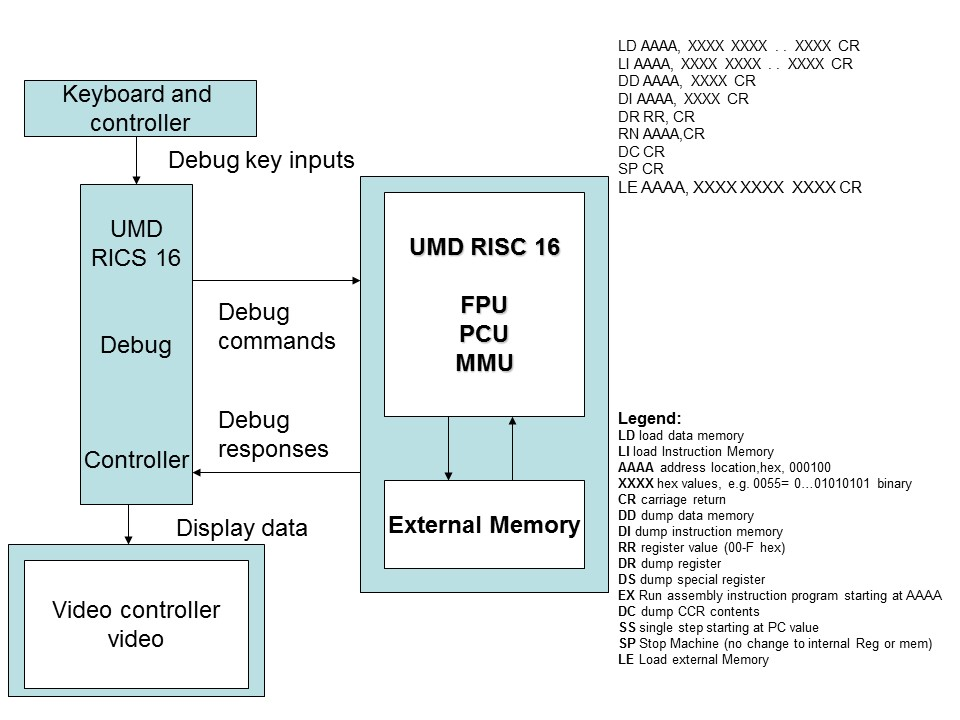
\includegraphics[width=0.7\textwidth]{images/RiscToplevel.jpg}}
  \caption{UMD RISC-16 Top Level I/O with debug conceptual architecture}
  \label{fig:RiscToplevel}
\end{figure}
\FloatBarrier

\begin{figure}[!htbp]
  \centering
      \fbox{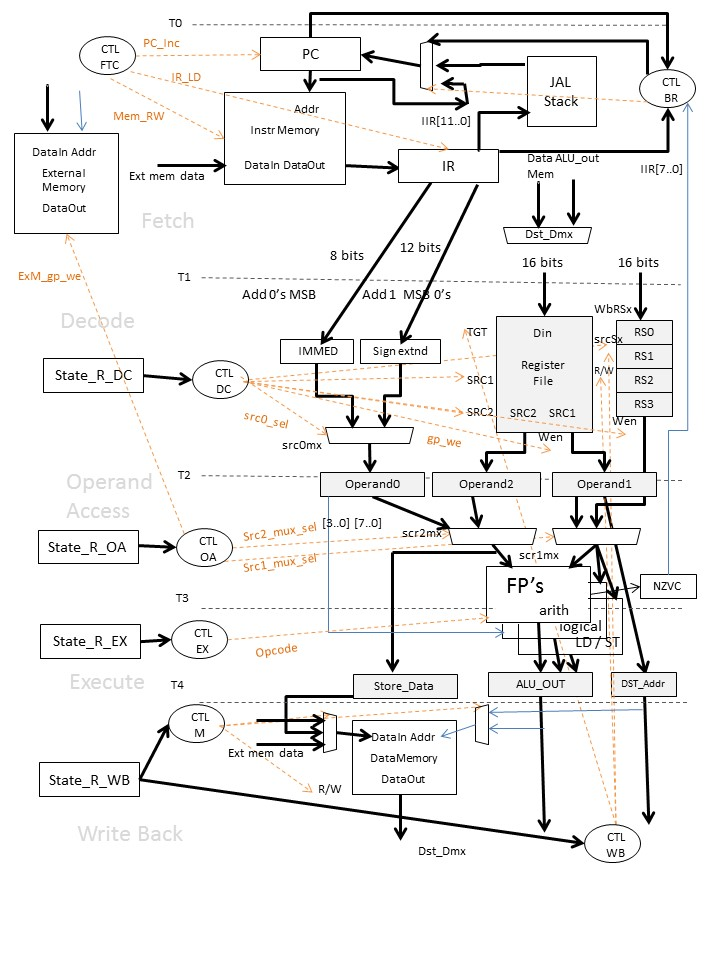
\includegraphics[width=0.7\textwidth]{images/UMDRISCLayout.jpg}}
  \caption{UMD RISC-16 Full data path and control unit RTL architecture}
  \label{fig:UMDRISCLayout}
\end{figure}
\FloatBarrier

\section{Procedure}

Follow the design procedure below to complete the lab. In this lab, you are required to create, document, and verify results of the test-benches and hardware test procedures you design and utilize in verifying and validating your design. Communicate which steps you were able to complete and the tests you used to ensure they operated as expected.

\begin{enumerate}

% Part 1
\item Table~\ref{tab:riscise} shows the desired instruction set for the UMD-RISC 16 machine to date. You are only required to add what is necessary for this lab at this current point. The shaded instructions are to be implemented for this lab to be successful. The LWV and SWV instructions will be necessary to demonstrate the functionality of your external memory unit that uses the Shadow registers. The JAL and RTL instructions will require implementing additional data path connections, a stack and additional controls. The BRA instruction will require the addition of an additional control element at a minimum and methods for stalling or flushing the pipe to support correct branch operations.

\begin{table}[!htbp]
\rowcolors{2}{gray!25}{white}
  \begin{center}
    \begin{tabular}{|c|l|l|}
       \hline
       \rowcolor{gray!50}
       \large{\textbf{OPCODES:}} & \large{\textbf{Operation:}} & \large{\textbf{Routine:}} \\
       \hline 
       \textbf{0000} & ADD  REG A, REG B & \specialcell{R[A] $\leftarrow$ R[A] + R[B] \\set status flags NZVC}  \\
       \textbf{0001} & SUB  REG A, REG B & \specialcell{R[A] $\leftarrow$ R[A] - R[B] \\set status flags NZVC}  \\
       \textbf{0010} & AND  REG A, REG B & \specialcell{R[A] $\leftarrow$ R[A] \& R[B] \\set status flags NZVC}  \\
       \textbf{0011} & OR   REG A, REG B & \specialcell{R[A] $\leftarrow$ R[A] $\mid$ R[B] \\set status flags NZVC}  \\
       \textbf{0100} & MOV  REG A, REG B & R[A] $\leftarrow$ R[B] \\
       \textbf{0101} & ADDI REG A, IMMED & \specialcell{R[A] $\leftarrow$ R[A] + IMMED \\set status flags NZVC}  \\
       \textbf{0110} & ANDI REG A, IMMED & \specialcell{R[A] $\leftarrow$ R[A] \& IMMED \\set status flags NZVC}  \\
       \textbf{0111} & SL   REG A, IMMED[0..3] & \specialcell{ R[A] $\leftarrow$  R[A\textless \textless IMMED] \\ zero fill LSB C and V affected}  \\
       \textbf{1000} & SR   REG A, IMMED[0..3] & \specialcell{R[A] $\leftarrow$ R[A\textgreater \textgreater IMMED] \\zero fill MSB}  \\
       \textbf{1001} & LW   REG A, IMMED[7..0] & R[A] $\leftarrow$ MEM[IMMED]  \\
       \textbf{1010} & SW   REG A, IMMED[7..0] & MEM[IMMED] $\leftarrow$ R[A]  \\
       \textbf{1011} & LWV  REG A, REG S, IMMED[7..0] & \specialcell{R[A] $\leftarrow$ ExMEM[R[S] + IMMED] \\when ID=00}  \\
       \textbf{1100} & SWV  REG A, REG S, IMMED[7..0] & \specialcell{ExMEM[R[S] + IMMED] $\leftarrow$ R[A] \\when ID=00}  \\
       \textbf{1101} & JAL  IMMED[16..0] & \specialcell{STK[SP+] $\leftarrow$ [PC],\\ PC $\leftarrow$ IMMED[16..0]}  \\
       \textbf{1110} & RTL & PC $\leftarrow$ STK[SP], SP $\leftarrow$ SP-1  \\
       \textbf{1111} & BRA MASK, IMMED[15..0] & \specialcell{PC $\leftarrow$ [PC]+ IMMED, \\if MASK \& NVZC is true}  \\
       \hline
    \end{tabular}
  \end{center}
  \caption{UMD RISC-16 Instruction Set Architecture}
  \label{tab:riscise}
\end{table}
\FloatBarrier

% Part 2
\item Create new components for use in your project for external memory access and jump and branching support.

Implementing external memory in RAMs in VHDL results synthesizing to LUTs rather than built in block RAMs, significantly increasing time to synthesize and implement, as well as slowly down the machine as a whole. To remedy this, Xilinx has built-in block RAMs that can be utilized. 

\textbf{Note:} You can ignore these if you like and implement the memories in any way you desire

% Part 3
\item Complete the remaining portions of the design. 

Much of the remaining support elements will consist of registers, multiplexers, new control states, etc. to be utilized for branching, jump and return operations.

% Part 4
\item Design an interrupt control utility.

For the interrupt controller you should design and build a controller that will monitor various signals in your design. One example of a interupt to look into is the change in state on a signal/pin (Pin change). The Interrupt controller you are developing should be its own unit. It will be up to you to choose a method for handling hardware generated signals.

% Part 5
\item Test loading a program from a file into your instruction memory and executing it.

A sample “.coe” file has been included for your reference. You will need to indicate that the memory will be loaded using a .coe file(\textbf{instruction\_memory.coe})

To load these into the instruction memory for the RISC machine to perform the following sequence of steps:


\begin{enumerate}
  \item Open instruction\_memory.coe in a text editor.
  \item The COE format is broken into 24 bit wide hex words per line, separated by commas. Each block of 8 words is separated by an additional newline. The instructions in the sample programs section are given in blocks of 8 to enter into this file. Simply, replace as many 24x8 blocks with the instructions given there and save the file.
  \item Open up the project in Xilinx IDE.
  \item In Sources for “Synthesis/Implementation” 
  \item Highlight “instruction\_memory\_block”, expand “Coregen” and run “Regenerate Core”
\end{enumerate}

When this is complete, the initialized contents of instruction memory will be that of the sample program.

%Part 6
\item Create a hardware debugging interface. 

Integrate the PS/2 keyboard and VGA (from Lab 3) as well as the debug unit (from Lab 4) into your design to support testing and debug of your design.

Required basic functionality includes displaying the contents of instruction and data memory, as well as manually changing values into memory in a manner you choose. Additionally, possibly supporting the ability to display contents of both the general purpose and special registers.

Be sure to document your hardware test procedure and report results clearly.

\end{enumerate}

\section{Deliverables}

Please only print out your top level code and any new component code created in this part of the project. A print out of all your code is not necessary. Please zip all VHDL files and UCF file and email to the \textbf{Instructor} and the \textbf{TA} with the filename \textbf{ECE368\_Project\_ Lab2\_Team\#.zip}. Describe your new VHDL designs in your lab report. You can use portions of the code or complete listings if necessary, but discuss how the components operate and any required conditions or constraints on them.

Explain your testbench, print out your testbench results, and discuss the results you observed. Likewise, explain your hardware test fully and discuss any final results and/or problems you encountered. Include any handwritten design flowcharts or pseudocode used in your lab report.

\section{Lab Report:}

Each lab group should prepare a lab report with the following information:
\begin{itemize}
  \item Follow the \textbf{CPE Laboratory Report Guidelines} for base format
  \item Machine RTL block level design
  \item VHDL component specification and schematic designs.
  \item VHDL system specification and resulting schematic design.
  \item Test plan design and test bench code
  \item Hardware test procedure used to verify your design
  \item Simulation results for your simple machine using a testbench (Prove it works).
  \item Schematic and UCF file for your simple machine.
  \item Conclusion needs to include a discussion of the learning utility of this lab and discussion of any issues you had with lab design and clarity.
  \item Reflection section discussing what you did well in your design, what you did not so good and why and what you plan to do to improve your design and design skills in the next lab and for the final project.
\end{itemize}

\section{Project Lab 2 Grade}

\begin{table}[!htb]
  \begin{center}
    \begin{tabular}[width=0.9\textwidth]{|l|c|l|}
       \hline
       Section & Value & Score\\
       \hline 
       \multicolumn{1}{|l}{\textbf{Procedure:}}  & -\textbf{60}- &\\
       \hline
       1. Implement External Memory Access(LWV,SWV) & 15 &\\
       \hline
       2. Implement Jump Support(JAL,RTL) & 15 &\\
       \hline
       3. Implement Branching Support(BRA) & 10 &\\
       \hline
       4. Design a Interrupt(INT) controller & 5 &\\
       \hline
       5. Test loading a program from a file & 5 &\\
       \hline
       6. Implement a Hardware Debugging Interface & 5 &\\
       \hline
       7. Show Final Hardware Test & 5 &\\
       \hline
       \multicolumn{1}{|l}{\textbf{Deliverables:}}  & -\textbf{20}- &\\
       \hline
       \multicolumn{1}{|l}{\textbf{Lab Report:}}  & -\textbf{20}- &\\
       \hline
       \hline
       \multicolumn{1}{|l}{Total} & \multicolumn{1}{c|}{100} &\\
       \hline
    \end{tabular}
  \end{center}
  \caption{Project Lab 2 Grade Breakdown}
\end{table}

\end{document}
